% Diese Zeile bitte -nicht- aendern.
\documentclass[course=erap]{aspdoc}
\usepackage{wrapfig}

%%%%%%%%%%%%%%%%%%%%%%%%%%%%%%%%%
%% TODO: Ersetzen Sie in den folgenden Zeilen die entsprechenden -Texte-
%% mit den richtigen Werten.
\newcommand{\theGroup}{141} % Beispiel: 42
\newcommand{\theNumber}{A208} % Be  ispiel: A123
\author{Aaron Tacke \and Philip Haitzer \and Thomas Sedlmeyr}
\date{Sommersemester 2020} % Beispiel: Wintersemester 2019/20
%%%%%%%%%%%%%%%%%%%%%%%%%%%%%%%%%

% Diese Zeile bitte -nicht- aendern.
\title{Gruppe \theGroup{} -- Abgabe zu Aufgabe \theNumber}

\begin{document}
	\maketitle
	
	\section{Einleitung}
	\subsection{Einsatz und Funktionsweise der Gammakorrektur}
	
	\begin{wrapfigure}{r}{0.35\linewidth}
		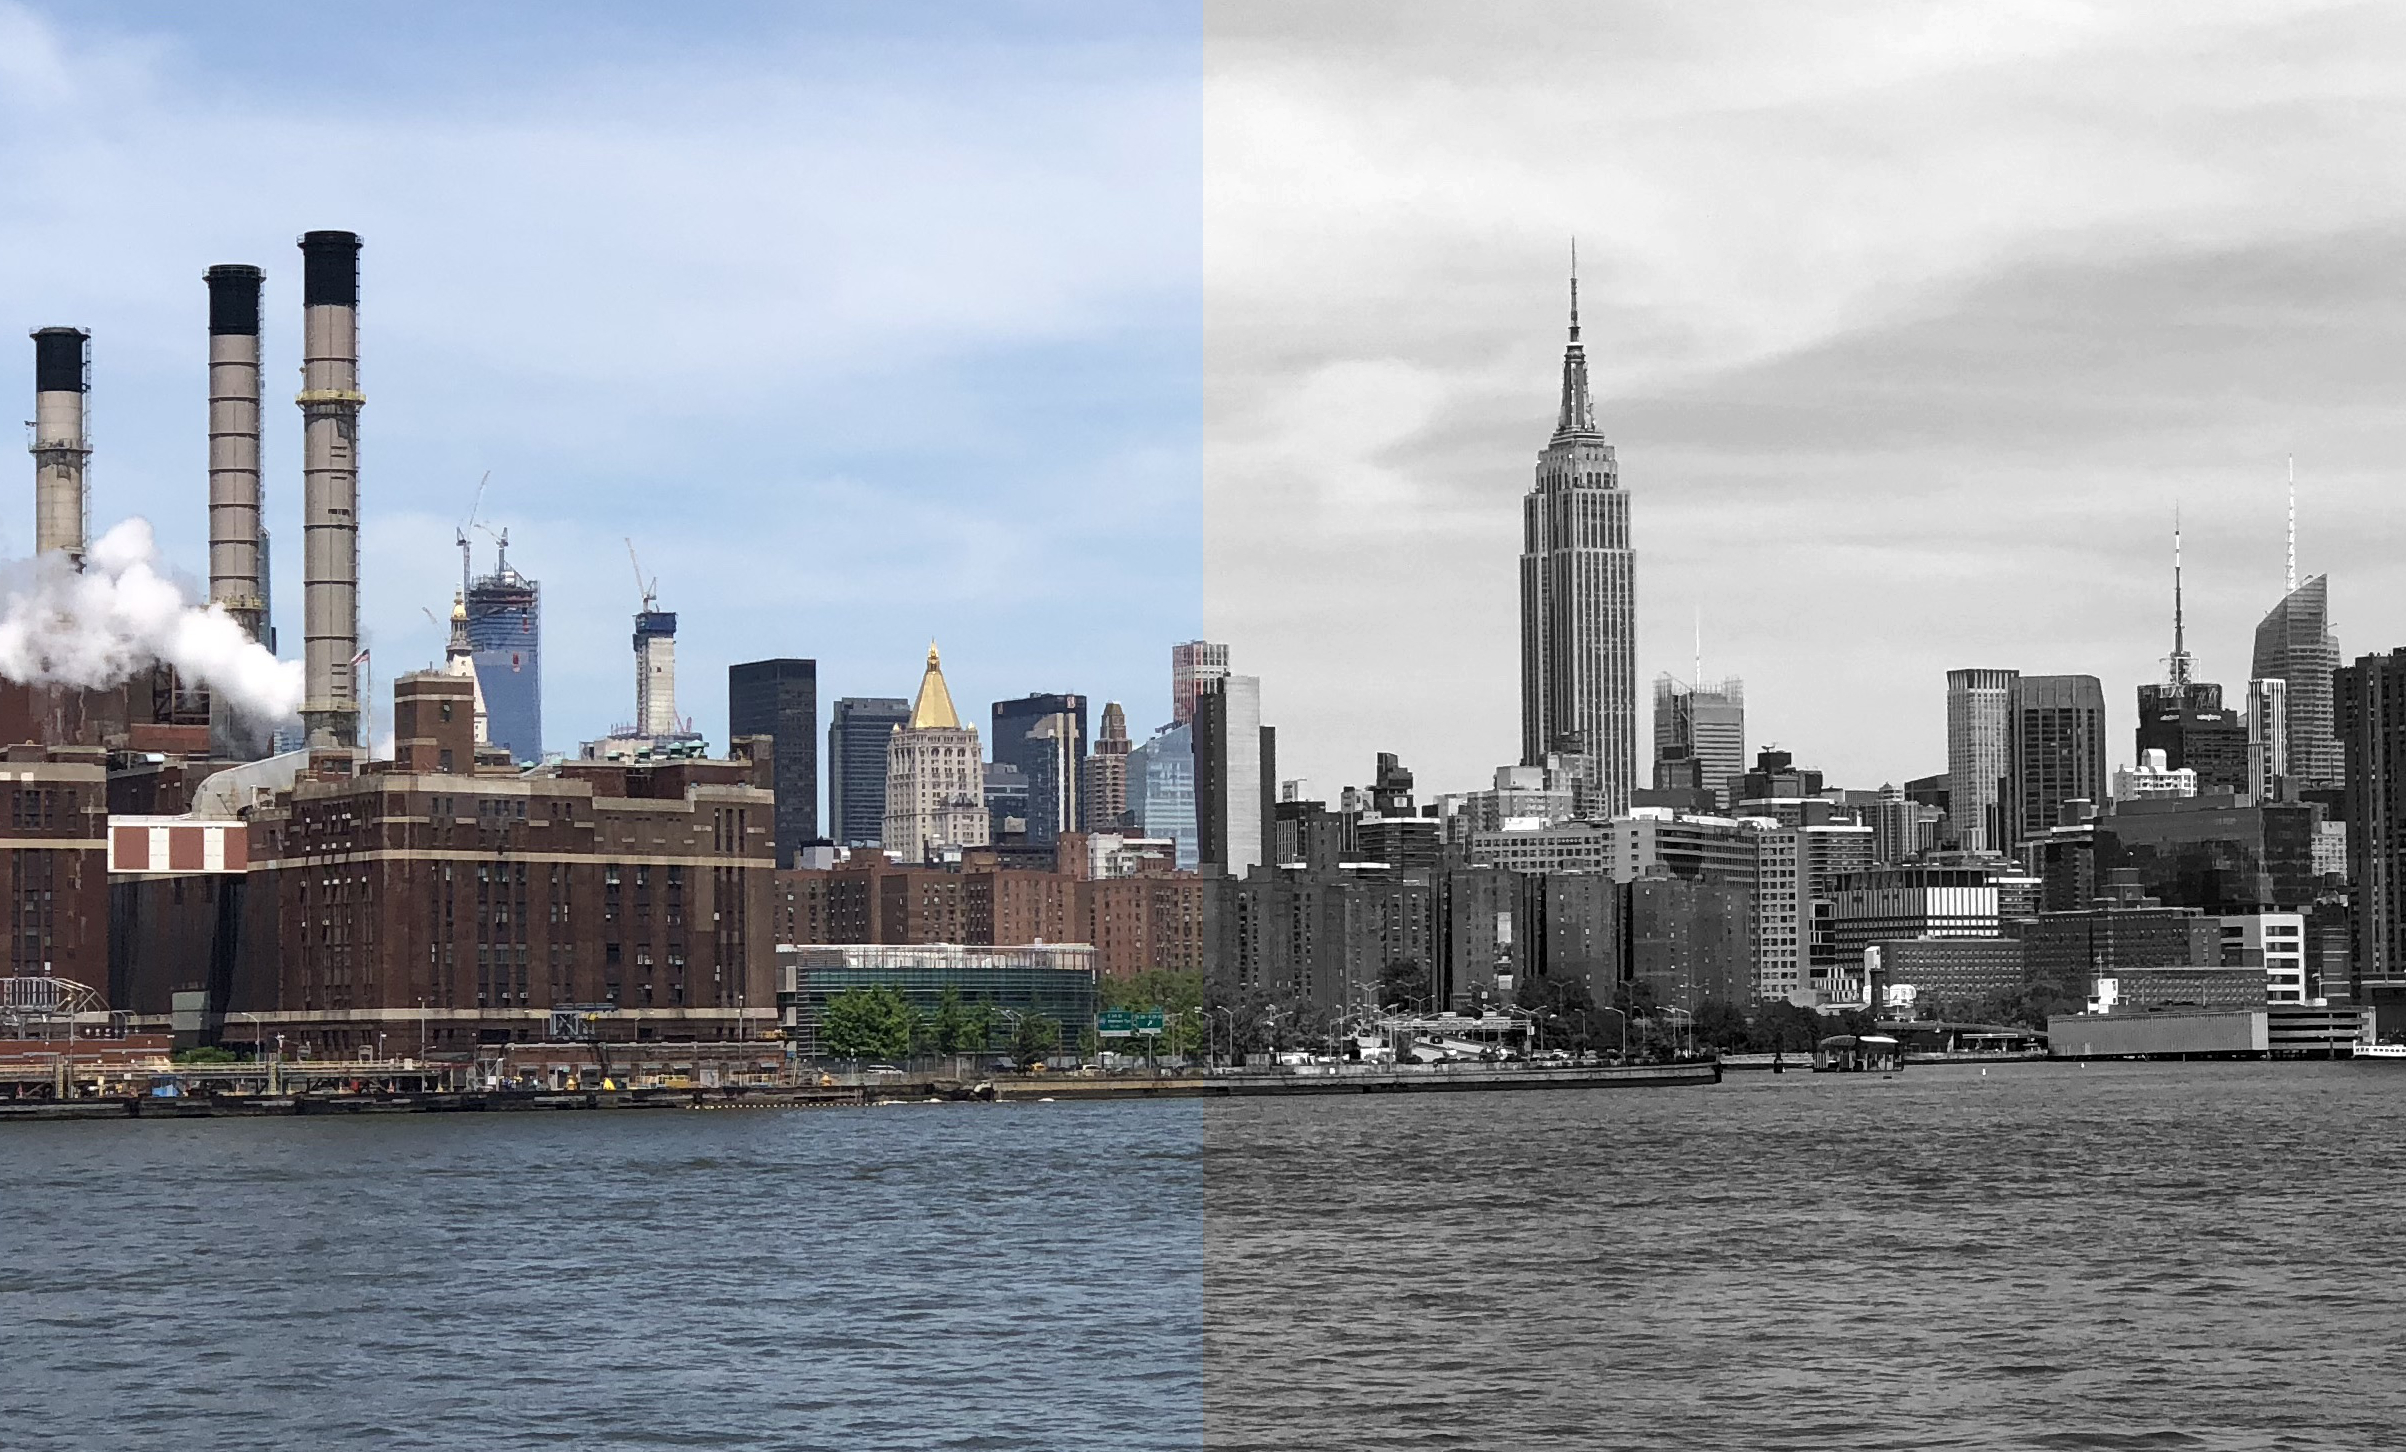
\includegraphics[width=5cm]{gammaBeispiel.jpg}
	\end{wrapfigure}
	Selbst über 100 Jahre nach der Entwicklung der Farbfotografie, erfreuen sich Schwarzweißbilder hoher Beliebtheit. Denn ohne störenden Farben lenken sie den Blick des Betrachters gezielt auf das Wesentliche und heben den Kontrast und die graphische Struktur der aufgenommenen Szenerie exzellent hervor.\\
	Um möglichst realistische Schwarzweisßbilder zu erzeugen, unterzieht man diese einer Gammakorrektur, bei der gezielt Einfluss auf die Helligkeit der einzelnen Pixel genommen wird.\\
	
	\noindent Möchte man mit heutigen Kameras digitale Schwarzweißaufnahmen machen, gelingt dies meist nur durch Umwandlung eines digitalen Farbbildes. Um trotzdem von der höheren Auflösung neuerer Fotografien zu profitieren, benötigen wir ein Programm, welches eine große Anzahl an Pixeln mit sinnvoll spezifizierten Gewichtungen der Farben in Graustufen umwandelt, und eine effiziente Gammakorrektur anwendet.\\
	
	\noindent Als Eingabe soll deshalb jedes ASCII-Kodierte Bild im PPM-Format, und eine vom Benutzer gewählte positive Fließkommazahl für die Gammakorrektur fungieren. Dabei soll die Ausgabe für jeden Gamma-Wert mathematisch korrekt berechnete Pixel liefern und diese in eine vom Benutzer spezifizierte Datei speichern.
	
	
	
	\section{Lösungsansatz}
	\subsection{PPM-Format}
	Die erste Zeile eines PPM-Bildes kennzeichnet das PPM-Format. Da wir mit Bildern, welche in ASCII gespeichert sind, arbeiten, erwarten wir hier "P3".
	Ein optionaler Kommentar ist in der zweiten Zeile zu finden.
	In der dritten Zeile werden Breite und Höhe des Bildes, durch ein Leerzeichen getrennt, angegeben.
    Die vierte Zeile enthält den maximalen Wert eines Farbanteils. Jede folgende Zahl liegt also zwischen 0 und dem hier spezifizierten Wert (einschließlich), welcher bei uns standardmäßig 255 sein muss.
    Danach folgen für jedes Pixel 3 Zeilen, welche die Rot-, Grün- und Blau-Werte für das jeweilige Pixel beinhalten.
	
	\subsection{Berechnung des Graustufenfilters}
	Zu Beginn wird jedes Pixel in Graustufen umgewandelt. Dabei berechnet sich der neue Wert eines Pixels mit folgender Formel.
	\begin{equation}
	\label{(2)}
	p_{alt} =  \begin{pmatrix}R \\\ G \\\ B \end{pmatrix} \qquad D = \frac{a \cdot R  + b \cdot G  + c \cdot B }{a + b + c} \qquad p_{neu} =  \begin{pmatrix}D \\\ D \\\ D \end{pmatrix}
	\end{equation}	
	% TODO: Birgt den vorteil, dass wir nicht divideren müssen
	Wir entschieden uns dafür, dass für die Gewichtung \begin{equation}
	a + b + c = 256
	\end{equation} gelten soll. Dies birgt den Vorteil, dass für die weitere Berechnung nur der Rest zu $256$ relevant ist und dieser durch einen Shiftbefehl effizient berechnet werden kann.
	
	\subsection{Optimierung des Graustufenfilters mit SIMD}
	Die Grundidee für die optimierte Berechnung mit SIMD ist es, mit Hilfe von drei xmm-Registern den Graustufenfilter auf fünf Pixel gleichzeitig anzuwenden. Hierfür werden jeweils der Rot-, Grün- und Blauanteil der Pixel in einem xmm-Register gespeichert, sodass sich vor jeder belegten Speicherzelle noch mindestens ein freies Byte befindet. Dann werden die xmm-Register jeweils mit zugehörigem Faktor ($a,b$ oder $c$) multipliziert. Im nächsten Schritt werden die xmm-Register aufaddiert und mit einer entsprechenden Bytemaske die niederwertigen Bytes der Ergebnisse extrahiert. Dies ist möglich, da $a,b$ und $c$ in Summe $256$ ergeben und durch die Maskierung der niederwertigen Bytes implizit der für die Division nötige Shiftbefehl ausgeführt wird.
	\\
	\newline
	\noindent
	Dabei stellten wir fest, dass die mit SIMD optimierte Ausführung weniger effizient verlief, als die Vergleichsimplementierung in C. Der Grund hierfür war, dass die Pixel nicht in 16 Byte Blöcken aligned waren und daher die Shiftbefehle für die richtige Anordnung der Pixelwerte in den xmm-Registern ca. $35\%$ der gesamten Berechnungsdauer benötigten. Aus diesem Grund sorgten wir für ein Alignment des Speichers, indem wir nach jedem 15. Byte ein 0 Bytes einfügten und die Assemblerimplementierung dementsprechend abänderten. Dabei ließen sich zudem ein paar Shiftbefehle einsparen und es gelang uns, mit der SIMD optimierten Version die Laufzeit um $x\%$ gegenüber des in C implementierten Graustufenfilters zu verbessern.  
	
	
	\subsection{Untersuchung der Gammafunktion}
	Unser Ziel ist es, für alle positiven Gammawerte, die mit dem Datentyp float darstellbar sind, die Gammakorrektur durchführen zu können.
	\begin{equation}
	p_{neu} = \left(\frac{p_{alt}}{255}\right)^{\gamma} \cdot 255
	\end{equation}   
	Da es sich bei $\gamma$ um eine Gleitkommazahl handelt, ist für diese Berechnung ein effizientes Berechnen und Potenzieren von Wurzeln erforderlich. Vor allem das Berechnen der n-ten Wurzel stellte sich als Problem heraus, weil hierfür eine Vielzahl an mathematischen Operationen ausgeführt werden müssen. Aus diesem Grund untersuchten wir die Gammafunktion hinsichtlich ihres Wertebereichs und Monotonieverhaltens, um ein effizienteres Verfahren zu entwickeln.
	\newline
	
	\subsection{Berechnung aller Gammafunktionen}
	Die zwei Erkenntnisse über die endliche Anzahl an unterschiedlichen Gammafunktionen und über das Monotonieverhalten nutzen wir, um mit Hilfe eines C-Programms Intervalle für $\gamma$ zu berechnen, in denen die jeweiligen Gammafunktionen für jeden Eingabewert von $0-255$ die gleiche Ausgabe liefern. Hierfür verwendeten wir Bisektion, indem mit zwei aufeinanderfolgenden float Werten gestartet und die Größe des Intervalls zunächst so lange verdoppelt wird, bis sich die Funktionswerte an den Intervallgrenzen unterscheiden. Von diesem neuen Intervall wird die Mitte und der Funktionswert an der mittleren Stelle berechnet. Ist dieser neue Wert gleich dem Funktionswert der rechten Intervallgrenze, wird das linke Intervall weiter verkleinert, wenn nicht wird das rechte verkleinert. Dies wird solange fortgeführt, bis die Stelle gefunden wurde, an der sich für zwei aufeinanderfolgende float Werte die Funktionswerte unterscheiden. Nach Ausführung des Programms speicherten wir die 64484 resultierenden Werte in einer Headerdatei ab, um bei späteren Tests über einfachen Zugriff zu verfügen.
	
	\subsection{Effiziente Speicherung von vorberechneten Gammafunktionen}
	Mittels Binärer Suche implementierten wir einen Algorithmus, der es ermöglicht für ein gegebenes $\gamma$ die vorberechnenten Werte der Gammafunktion zu bestimmen.  Dabei stellte sich aber heraus, dass die Zeit für das Kompilieren der großen Headerdatei ca. eine halbe Minute in Anspruch nahm. Aus diesem Grund beschäftigten wir uns damit, wie eine effizientere Speicherung von Gammafunktionen aussehen könnte, um weniger Daten abspeichern zu müssen und die Compilezeit zu verkürzen.
	\\
	\newline
	\noindent
	Für die Optimierung des Speicherplatzes nutzten wir die Monotonieeigenschaft der Gammafunktion. Da diese monoton steigend ist, reicht es aus, abzuspeichern, um wie viel der nächste y-Wert größer ist als der vorherige. Dies bedeutet, dass sich jede Gammafunktion binär repräsentieren lässt, indem die Anzahl der Nullen vor der nten $1$ den nten Funktionswert liefern. Abbildung \ref{KompremierungBeispiel} zeigt ein Beispiel für die ersten sechs Werte einer Gammafunktion. 
	
	
	\noindent
	\begin{wrapfigure}{r}{0cm}
        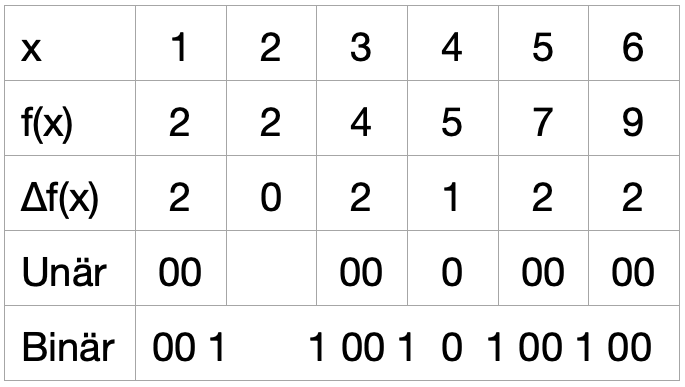
\includegraphics[width=9cm]{Images/CompressionOfFunctions.png}
         \caption{Bildunterschrift}
         \label{KompremierungBeispiel}
    \end{wrapfigure}
	Da die Gammafunktionen jeweils nur 256 Funktionswerten aus dem Wertebereich zwischen $0$ und $255$ besitzen, benötigt man 256 Einsen und 256 Nullen, um eine Gammafunktion abzuspeichern. Dies bedeutet, dass sich mit 64 Byte, also mit vier Zahlen des Datentypes $\_\_int128$, eine Gammafunktion abspeichern lässt. Da wir aber keine einfach Möglichkeit fanden, Zahlen des Datentyps $\_\_int128$ in einen String zu konvertieren und sich zudem das Dekodierem mit Xmm-Registern als schwierig erwies, speicherten wir die kodierte Funktion mit acht Dezimalzahlen des Datentypes $long long$ ab. Mit diesem Verfahren gelang es uns, den Speicherverbrauch von zuvor 70MB Bytes auf ein siebtel zu reduzieren und die Compilezeit von zuvor 17 Sekunden auf zwei Sekunden zu senken. 
	Abbildung \ref{KompremierungBeispiel} zeigt anhand einer Beispielfunktion das Kompressionsverfahren. Diese Funktion würde mit $001100101001001_{2}$ als Binärzahl oder mit $6473_{10}$ im Dezimalsystem repräsentiert. 

	\subsection{Decodierung der Komprimierten Funktionen}
	Für das Decodieren einer so komprimierten Funktion werden für den jeweils vom Benutzer spezifizierten Gammawert die acht zugehörigen Werte aus dem Speicher der Reihe nach geladen und Bitweise nach links geshiftet. Nach jedem Shiftbefehl wird mit Hilfe des Carry-Flags überprüft, ob eine Null oder Eins aus dem Register geshiftet wurde und der jeweilige Zähler erhöht. Wenn es sich um eine Eins handelt, bedeutet dies, dass der Funktionswert für x = Zähler der Einsen, der Anzahl der bisher gezählten Nullen entspricht. Dieser Wert wird abgespeichert und der Algorithmus solange wiederhohlt, bis die gesamten 512 Bit durchgeshiftet wurden. Mit diesem Verfahren werden für einen Gammawert die Funktionswerte aller möglichen $x\in{1,...,255}$ vorberechnet.

	\subsection{Berechnung der Wurzel}
	Eine weitere Methode, um die für die Gammafunktion benötigte Wurzel $\sqrt[n]{z}$ zu berechnen, ist es, diese als Nullstelle des Polynoms $f(x)=x^n-z$ auszudrücken und diese mit verschiedenen Verfahren zur Nullstellenapproximation wie zum Beispiel dem Newtonverfahren anzunähern. Weil man aber selbst für das schnell konvergierende Newtonverfahren mehrmals verschiedene Funktionswerte von $f(x)$ berechnen muss, stellte sich dieses Verfahren als nicht effizient genug heraus.     
	
	\subsection{Binäre Suche zur Berechnung der Gammafunktion}
	Um die Gammafunktion zu berechnen, wandelten wir  $\gamma$ in einen Bruch bestehend aus zwei Integern um. Ziel dieses Verfahrens war es wieder mit Hilfe von Binärer Suche den richtigen Wert der Gammafunktion zu bestimmen, indem ...Aaron
	\\
	\newline
	\noindent	
	Zur Berechnung der ganzzahligen Potenzen implementierten wir zudem eine Methode, die es ermöglicht mit Hilfe von Binärer Exponentiation die Anzahl, der für die Potenzierung erforderlichen Multiplikationen, auf ein Minimum zu reduzieren. 
	\\
	\newline
	\noindent		 
	Für einen Großteil der Werte von $\gamma$ erwies sich diese Verfahren als effizient. Aber die Genauigkeit des Bruchs für die Darstellung von $\gamma$ wies kleine Fehler auf, die sich durch das Potenzieren aufsummierten, sodass es bei manchen $\gamma$ Werten zu Fehlern bei der Berechnung kam.       
	
	\subsection{Berechnung auf den Exponenten}
	Um die Umwandlung von Dezimalzahlen in Brüche zu umgehen, formten wir mit Hilfe der Logarithmusgesetze die Gammafunktion um. ...Aaron
	\begin{align}	
	p_{neu} = \left(\frac{p_{alt}}{255}\right)^{\gamma} \cdot 255
	\end{align}
	\begin{align}	
	\ln (p_{neu}) = \gamma \cdot \ln\left(\frac{p_{alt}}{255}\right) \cdot \ln(255)
	\end{align}
	\begin{align}
	p_{neu} \cdot 255^\gamma = {p_{alt}}^{\gamma}
	\end{align}
	\begin{align}
	\gamma \cdot \ln ( p_{neu} \cdot 255) = \gamma \cdot \ln({p_{alt}})
	\end{align}
	
	\subsection{Vergleichsimplementierung}
	Die Vergleichsimplementierung nutzt die Funktionen der C-Standardbibliothek um die Pixel nacheinander mit den angegebenen mathematischen Funktionen zu berechnen. Trotz Kompilierung mit -O3 haben wir die Laufzeit dieser Implementierung so exterm unterboten, dass wir eine zweite Vergleichsimplementierung erstellt haben, welche auf die Funktionswerte aller möglicher vorher berechneter Funktionen im Speicher zugreifen kann, und statt des langsamen Potenzierens lediglich die passende Funktion binär suchen musste. Wir haben mit dieser Methode zwar noch kein falsches Ergebnis feststellen können, allerdings ist die vollständige Korrektheit schwer zu beweisen, und die berechneten Funktionen führen zu langsamen Compile-Zeiten und großen ausführbaren Dateien, weshalb sie lediglich zum Benchmarking, nicht jedoch in der finalen Version des Programmes eingesetzt wurde.
	\subsection{Intuitve Bestimmung des Graustufenfilters}
	Die einfachste Form des Graustufenfilters, bei der nur der Durchschnitt der einzelnen Farbwerte mit Hilfe von (1) berechnet wird, nutzt $a=b=c=1$ als Parameter. Bei dieser einfachen Umwandlung wird jedoch fälschlicherweise angenommen, dass alle Farben vom menschlichen Auge gleich hell wahrgenommen werden. Die eigentliche Farbwahrnehmung unterscheidet sich jedoch von dieser Vorstellung, da beispielsweise die Farbe grün heller wahrgenommen wird als blau. Um diese Informationen bei der Umwandlung in Graustufen beizubehalten, müssen die Parameter a, b und c so angepasst werden, dass die Helligkeit in dem Graustufenbild der menschlichen Wahrnehmung der Farben auf dem ursprüglichen Bild entspricht.
	\begin{figure}[h]
		\begin{minipage}{0.49\linewidth}
			\centering
			%TODO funktioniert mit fruit_basket_original.png ganz normal, muss aber grey_standard sein
			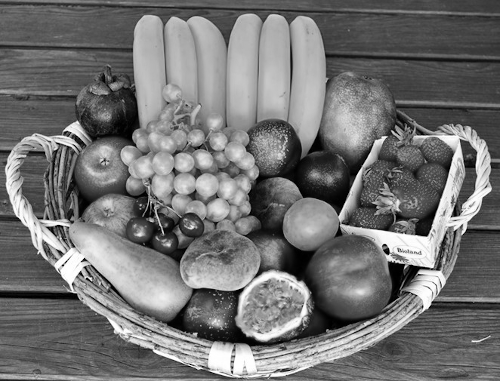
\includegraphics[scale=0.3]{Images/fruit_basket_grey_standard.png}
			\caption{Ohne Gewichtung}
		\end{minipage}
		%\hfill
		\centering
		\begin{minipage}{0.49\linewidth}
			\centering
			%TODO funktioniert mit fruit_basket_original.png ganz normal, muss aber grey_improved sein
			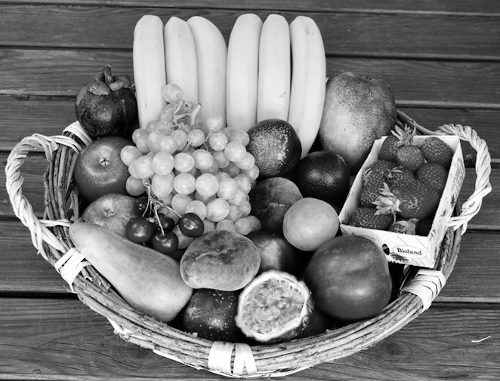
\includegraphics[scale=0.3]{Images/fruit_basket_grey_improved.png}
			\caption{Mit Gewichtung}
		\end{minipage}
	\end{figure}
	Im Vergleich der beiden Bilder ist zu erkennen, dass die Farben mit einer sinnvollen Gewichtung des Graustufenfilters viel realistischer in Graustufen umgewandelt werden. So sind die als heller wahrgenommenen Farben wie gelb oder grün auch in dem Graustufenbild deutlich heller dargestellt und lassen sich somit besser von den anders farbigen Objekten unterscheiden. In dem ersten Bild hingegen lässt sich kein eindeutiger Farbunterschied zwischen den einzelnen Früchten erkennen. Es ist somit deutlich, dass die Wahl der Paramter eine entscheidende Rolle für die realistische Umwandlung eines farbigen Bildes in Graustufen spielt. Wie ein möglichst idealer Wert, der nicht nur auf Intuition basiert, sondern an die menschliche Farbwahrnehmung angepasst ist, bestimmt werden kann, wird im Folgenden erläutert.
	\subsection{Anpassung des Graustufenfilters auf das menschliche Auge}
	Um den Einfall von Licht wahrzunehmen, befinden sich in der Retina des Auges sogenannte Stab- und Zapfenzellen, beide eine Art modfizierte Nervenzelle, welche Photonen (Licht) absorbieren können, und ein entsprechendes elektrisches Signal Richtung Gehirn weiterleiten.
	Die Farbwahrnehmung beider lässt sich durch eine sogenannte Absorptionskurve beschreiben, welche angibt, welche Wellenlängen (Farben) am stärksten absorbiert, in elektrische Signale umgewandelt und somit wahrgenommen werden.
	Zapfenzellen erzeugen bei guter Beleuchtung scharfe Bilder, wohingegen Stabzellen für das Sehen bei geringem Licht und in peripheren Blickwinkeln verantwortlich sind. Somit müssen wir uns für die Wahl der Gewichtung von Farben für den Graustufenfilter lediglich an der Absorptionskurve von Zapfenzellen orientieren.
	
	\subsection{Resultate bei unterschiedlichen Gammawerten}
	Die Empfindung von Helligkeit des menschlichen Auges ist logarithmisch und folgt wie viele anderen neurologische Prozesse dem Weber-Fechner-Gesetz \cite{weberFechnerGesetz}. In dunklen Bereichen steigt die Helligkeitssensitivität stärker an \cite{Logarithmische_Helligkeitswahrnehmung}. Durch die richtige Wahl von $\gamma$ können die Grauwerte eines Bildes gezielt so verändert werden, dass für das menschliche Auge realistischer wahrgenommen werden. 
	\\
	\newline
	Ein weiterer Vorteil der Gammakorrektur besteht in der Aufhellung oder der Abdunklung von Fotos. So werden durch die Gammafunktion die dunkleren Pixel stärker aufgehellt als die die helleren Pixel. \cite{gammKorrekturWikipedia}
	Dadurch bleibt das Helligkeitsspektrum erhalten und das Bild wirkt realistischer. 
	\\
	\newline
	Im Folgenden sind mehrere Bilder zu sehen auf die Gammakorrekturen mit unterschiedlichen Werten für $\gamma$ angewendet worden sind, um die Wirkung der Gammafunktion zu demonstrieren.  
	
	\begin{figure}[h]
		\begin{minipage}{0.49\linewidth}
			\centering
			\includegraphics[scale=1.2]{Images/fruit_basket_gamma_1.png}
			\caption{Ohne Gammakorrektur}
			\label{ObstkorbGamma1}
		\end{minipage}
		%\hfill
		\centering
		\begin{minipage}{0.49\linewidth}
			\centering
			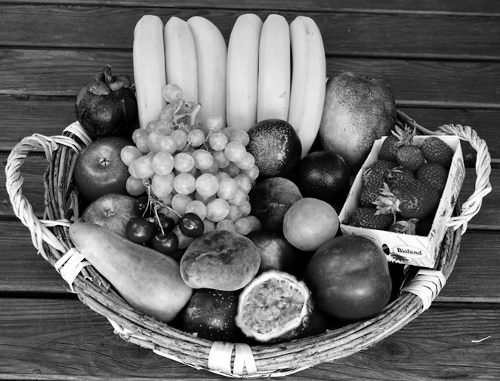
\includegraphics[scale=1.2]{Images/fruit_basket_gamma_1,25.png}
			\caption{Korrektur mit $\gamma = 1,25$}
			\label{ObstkorbGamma1_25}
		\end{minipage}
		%\hfill
		\begin{minipage}{0.49\linewidth}
			\centering
			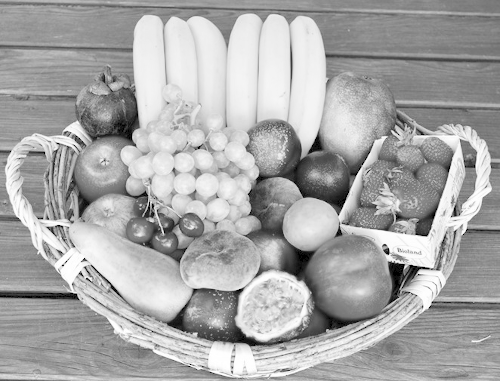
\includegraphics[scale=1.2]{Images/fruit_basket_gamma_0,5.png}
			\caption{Korrektur mit $\gamma = 0,5$}
			\label{ObstkorbGamma0_5}
		\end{minipage}
		%\hfill
		\centering
		\begin{minipage}{0.49\linewidth}
			\centering
			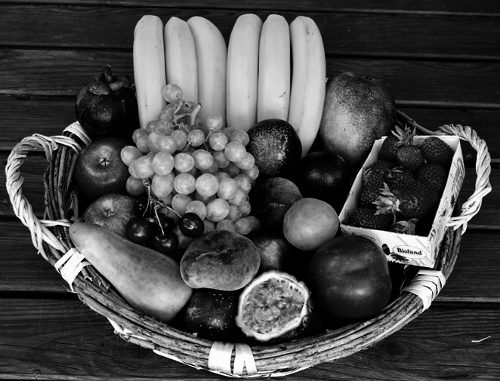
\includegraphics[scale=1.2]{Images/fruit_basket_gamma_2.png}
			\caption{Korrektur mit $\gamma = 2.0,$}
			\label{ObstkorbGamma2}
		\end{minipage}
	\end{figure}
	
	
	\noindent
	An den Bildern ist zu erkennen, dass für $\gamma > 1$ die Bilder dunkler werden und sich der Kontrast erhöht. Dieser Effekt lässt sich am besten Verstehen, wenn man die zugehörigen Graphen der unterschiedlichen Gammafunktionen betrachtet. So verlaufen alle Graphen mit $\gamma < 1$  unter dem Graphen $f(x)=x$. Dies bedeutet der Grauwert wird kleiner und das Bild wird dunkler dargestellt. Alle Funktionen mit $\gamma ' = \frac{1}{\gamma}$ stellen die Umkehrfunktion zur Funktion mit $\gamma$ dar und sind deshalb symmetrisch zur Winkelhalblierenden des ersten Quadranten. Daher verlaufen diese Funktionen oberhalb des Graphen von $f(x)$ und liefern größere Grauwerte. Das bearbeitete Bild wird daher heller dargestellt. Wenn man für $\gamma$ den Wert $1,25$ wählt, erhält man ein Bild dessen Kontrast der sehr realistisch wirkt siehe Abbildung \ref{ObstkorbGamma1_25}.   
	
	\noindent
	Zudem ist interessant, dass die Gammafunktion nicht jeden Grauwert gleich stark verändert. Abbildung 5 zeigt um wie viel sich die Helligkeit eines Pixels durch die jeweilige Gammafunktion verändert. Da es sich hier um keinen konstanten Wert handelt, werden zu Beispiel für $\gamma = 0.5$ die dunklen Pixel stärker aufgehellt als die hellen. Dies erzeugt einen besseren Kontrast??????
	\newline
	Der perfekte Wert für $\gamma$ lässt sich im Vorfeld nicht bestimmen, denn dieser ist abhängig von der Belichtung und dem Kontrast des aufgenommenen Fotos.
	\begin{figure}[h]
		\begin{minipage}{0.49\linewidth}
			\centering
			\includegraphics[scale=0.75]{Images/GammafunctionsDistanceToX.PNG}
			\caption{Korrektur mit $\gamma = 0,5$}
			\label{imageDistance}
		\end{minipage}
		%\hfill
		\centering
		\begin{minipage}{0.49\linewidth}
			\centering
			\includegraphics[scale=0.75]{Images/GammafunctionsPlotFor2And0,5.PNG}
			\caption{Korrektur mit $\gamma = 2.0,$}
			\label{GammafunctionsPlot}
		\end{minipage}
	\end{figure}
	\section{Korrektheit/Genauigkeit}
	\subsection{Berechnung aller möglichen Gammafunktionen}
	Uns war es wichtig, für jedes positives $\gamma$, das mit einem float dargestellt werden kann, den korrekten Wert zu berechnen und so die Berechnung nicht unnötig einzuschränken. Da wir alle möglichen Gammafunktionen kennen, können wir für unser Programm garantieren, dass jeder $\gamma$ Wert korrekt berechnet wird. 
	\\
	Auch verglichen wir alle Resultate der Assemblerimplementierungen mit äquivalenten C-Implementierungen, um sicherzugehen, dass die Optimierungen keine Fehler hervorriefen.  
	\subsection{Robustheit des Programms}
	Unser Programm prüft zudem, ob die übergebene ppm-Datei fehlerhaft ist und fängt falsche Parameter des Benutzers wie zum Beispiel negative $\gamma$ Werte oder nicht unterstütze Operationen ab. 
		\section{Zusammenfassung und Ausblick}
	
	
	% TODO: Fuegen Sie Ihre Quellen der Datei Ausarbeitung.bib hinzu
	% Referenzieren Sie diese dann mit \cite{}.
	% Beispiel: CR2 ist ein Register der x86-Architektur~\cite{intel2017man}.
	\bibliographystyle{plain}
	\bibliography{Ausarbeitung}{}
	\printbibliography
\end{document}
